\chapter{Background from the main beam dumps}
\label{BeamDumps}

\begin{chapterabstract}
 After every beam collision, the beams of a linear collider are dumped into the main beam dumps.
 For the International Linear Collider, the main beam dump design is based on a water tank, which is tailored to absorb the beam power over a length of about \textit{\SI[detect-all]{12}{\meter}}.
 The first part of this chapter is focused on the irradiation of the water tank and its surrounding, as well as on the neutrons that are produced due to the interaction of the beam particles with the water molecules.
 The second part of this chapter discusses those neutrons which are directed backwards and reach the interaction region.
 They present an additional background for the experiments.
 In the end, suggestions for alternative beam dump designs are given.
\end{chapterabstract}

The spent \positron\electron beams are directed through the extraction line (EXT) of the ILC towards the main beam dumps. 
As can be seen in Figure~\ref{fig:BeamDumps:IP_to_Dump}, the beam dump halls are about \SI{300}{\meter} away from the interaction point (IP) in a direct line of sight.
The extraction lines have the task to transport the highly disrupted beams to the dumps, because of which their quadrupole magnets have a large acceptance for offsets in the beam orbit as well as in the beam momentum of up to \SI{60}{\percent}~\cite[p. 139]{TDR32}.
The quadrupole magnets are to minimize beam loss so that additional diagnostic devices in the EXT lines can measure the qualities of beam bunches before they are dumped.
\begin{figure}
\centering
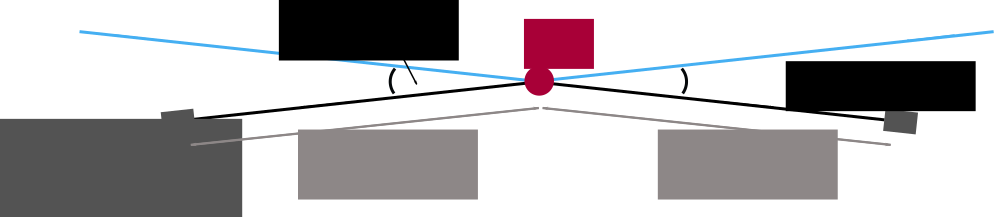
\includegraphics[width=0.6\textwidth]{Figures/BeamDump/IP_EXT.png}
\caption[Schematic of the ILC interaction region with extraction line]{Illustration of the interaction region of the ILC with the extraction line (EXT) leading from the IP to the main beam dump halls.
The extraction lines are about \SI[detect-all]{300}{\meter} long.
The illustration is not to scale.}
\label{fig:BeamDumps:IP_to_Dump}
\end{figure}
\\The beam dump designs are based on water tanks, which are surrounded by iron and concrete shielding walls. 
The two different designs, which are studied in this chapter, are described in detail in Section~\ref{BeamDumps:designs}.
The choice of a water tank as the beam dump is motivated by the high specific heat capacity of water, which is ideal to dissipate the energy of the beams. 
The water beam dumps for the ILC have to be able to absorb a beam power of up to about \SI{17}{\mega\watt}\footnote{This value includes the average beam power of \SI{13.7}{\mega\watt} at a center-of-mass energy of \SI{1}{\TeV} plus safety margins of \SI{20}{\percent}.} for the ILC stage at a center-of-mass energy of \SI{1}{\TeV}~\cite{BeamDumpSpecs}.
\\The high energy lepton beam interacts with the water molecules, leading to the emission of neutrons under all solid angles. 
Not only the effect of these neutrons reaching back to the interaction region, but also the doses that the surrounding area would suffer from, are the center of interest in this chapter. 
The rise in the occupancy of the detector experiments is one effect of the neutrons, whereas the damage of the detector components is another severe consequence.
The neutron background would on the one hand lead to displacement damage in the silicon sensors, which results in charge traps, reduction of charge transfer and the overall degrading of the detector performance. 
On the other hand, the immediate irradiation of the beam dump surrounding leads to restricted access for the maintenance staff and personnel.
\\It is therefore crucial to understand the irradiation and the level of neutron background generated by every beam pulse dumped into the ILC main beam dumps.

\section{\fluka and \flair}
\label{BeamDumps:fluka}
The simulation study of the ILC main beam dumps for this thesis was done using the Monte Carlo simulation tool \fluka~\cite{FLUKA,FLUKA2}.
\fluka calculates the particle transport and interactions with matter of the user-defined geometry.
With the graphical interface \flair~\cite{FLAIR}, which was specifically developed for \fluka, complex geometries can be constructed with the help of technical drawings that can be imported as templates into the \flair-geoviewer plug-in (see Figure~\ref{fig:BeamDumps:geoviewer}).
It allows interactive geometry viewing and editing, as well as debugging and three dimensional visualization.
\\\fluka's capabilities cover furthermore the calculation of particle densities and energy densities, the activation of material, and the residual dose rates when considering variable cooling times.
These functionalities were used for the study of the ILC beam dump designs presented in the following sections.
\begin{figure}[hbp]
\centering
\includegraphics[width=0.5\textwidth]{Figures/BeamDump/Design2_geometry_drawing_xz.png}
\caption[Preview of the geometry construction in \flair]{Preview of the construction of the ILC beam dump using a technical drawing as a template imported into the \flair-geoviewer plug-in.}
\label{fig:BeamDumps:geoviewer}
\end{figure}

\section{ILC main beam dump designs}
\label{BeamDumps:designs}
The designs for the main beam dump in this study are based on the technical design drawings done by Benjamin Smith~\cite{Smith_drawings}.
The drawings include plans for the surface building, the beam dump hall with the shielding walls around the water tank, and two different designs for the main beam dumps.
The design based on the drawing with the identification number 0-TB-0067-210-00-A shall henceforth be called ``\designone'', the second design based on drawing 0-TB-0067-300-00-A shall be called ``\designtwo''.
Figure~\ref{fig:BeamDumps:geometry} shows a visualization of the beam dump hall modeled within \flair. 
The innermost shielding wall around the beam dump vessel is made of iron, and has a thickness of \SI{50}{\centi\meter}.
The middle layer of shielding consists of \SI{1.5}{\meter} thick boronated concrete, surrounded by a layer of normal concrete, which has a thickness of \SI{2}{\meter}.
Boronated concrete is enriched with boron for the specific purpose of radiation shielding.
The composition of both concrete types, boronated and normal, was adapted from concrete mixtures used in Japanese research centers, as described in~\cite{concrete}. 
The infrastructure, such as cables and water pipes, is not included in the simulation geometry.
\\As mentioned in the section above, technical design drawings can be imported into \flair, and directly used as templates for the construction of the geometry.
This was done for the two beam dump designs, which will be explained in detail in the following.

\begin{figure}[hbp]
\begin{center}
\resizebox{.9\textwidth}{!}{%
\includegraphics[height=0.35\textheight]{Figures/BeamDump/Front_view_BeamDump_Tomb.png}%
\quad
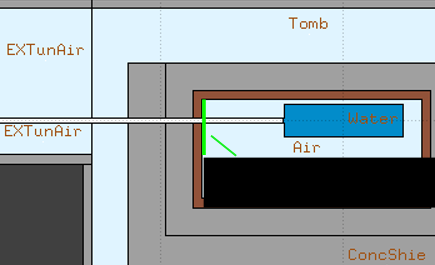
\includegraphics[height=0.35\textheight]{Figures/BeamDump/Bird_view_BeamDump_Tomb.png}%
}
\caption[Geometry visualization of the ILC main beam dump hall]{Simplified version of the beam dump hall for the purpose of visualization, containing only a simple water tank in the middle of the shielding walls. 
The geometry was modeled within \flair according to the technical drawings of the ILC beam dump facility.
The left hand picture is the front view, the beam direction is going into the page.
The right hand figure shows the top view, in which the water tank is shown in the middle of the different shielding walls. 
A \fluka specific feature is the need of having a black body void around the geometry. 
This void is the boarder of the tracking region, and stops all particles reaching this edge.}
\label{fig:BeamDumps:geometry}
\end{center}
\end{figure}

\subsection{\designone}
\label{BeamDumps:design:design1}
As both beam dump designs are based on a water tank system, their basic layout is very similar.
For both, the water vessel out of 316L stainless steel has a diameter of \SI{1.5}{\meter} and a length of \SI{6.5}{\meter}.
The water is pressurized to \SI{10}{\bar}.
The window between the vessel and the beam pipe has a diameter of \SI{30}{\centi\meter} and a thickness of \SI{1}{\milli\meter}.
For its material, the titanium alloy Ti-6Al-4V is foreseen.
\\As can be seen from Figure~\ref{fig:BeamDumps:design1}, the vessel contains an inner vortex system.
The turbulence of the water allows the arising heat from the beam power to dissipate.
\\Overall, the water volume represents a radiation length of \SI{18}{\xzero}.
Additional \SI{9}{\xzero} are placed in the end of the vessel in form of water cooled copper plates.

\begin{figure}[h]
 \centering
  \begin{subfigure}[b]{0.49\textwidth}
   \centering
    \includegraphics[width=\textwidth]{Figures/BeamDump/TB-0067-210-00-A_yz_view.png}
   \caption{Technical drawing, yz view}
   \end{subfigure}
   \hfill
    \begin{subfigure}[b]{0.49\textwidth}
   \centering
    \includegraphics[width=\textwidth]{Figures/BeamDump/Design1_geometry_3Dinside.png}
   \caption{\fluka model, 3D view}
   \end{subfigure}
   \caption[ILC main beam dump design 1]{Figure (a) shows the yz view of the beam dump \designone from the technical drawing.
   The \fluka model constructed within \flair is shown in Figure (b).}
   \label{fig:BeamDumps:design1}
 \end{figure}

\subsection{\designtwo}
\label{BeamDumps:design:design2}
The basic layout explained above for \designone was also adopted for \designtwo, so that the measurements of the vessel and the window are the same for both designs.
The main difference is the addition of a high pressure water section in the middle of the vessel  for \designtwo.
Figure~\ref{fig:BeamDumps:design2} shows the 3D model of \designtwo implemented within \flair, with the high presser water section in the middle. 
The titanium tubes of this system have a diameter of \SI{4}{\centi\meter}, through which high pressure water is pumped.
\\The vortex system shows also a different design approach.
More tubes are connecting the vortex system with the outside pumps.
The copper plates, however, are also in this design placed in the end of the vessel for additional radiation length.

\begin{figure}[h]
 \centering
  \begin{subfigure}[b]{0.49\textwidth}
   \centering
    \includegraphics[width=\textwidth]{Figures/BeamDump/Design2_geometry_3Dinside3.png}
   \caption{\fluka model, yz view}
   \end{subfigure}
   \hfill
    \begin{subfigure}[b]{0.49\textwidth}
   \centering
    \includegraphics[width=\textwidth]{Figures/BeamDump/Design2_geometry_3Dinside1.png}
   \caption{\fluka model, 3D view}
   \end{subfigure}
   \caption[ILC main beam dump design 2]{Figure (a) shows the yz view of the \fluka model of the beam dump \designtwo, the 3D view is shown in Figure (b).}
   \label{fig:BeamDumps:design2}
 \end{figure}

\section{Simulation studies of the beam dump surrounding}
\label{BeamDumps:sim_surrounding}
For the \fluka simulation of the ILC beam being dumped into the water tanks of \designone and \designtwo as explained above, the running scheme of the ILC1000B~\cite[p. 11]{TDR1} stage was chosen.
The beam bunches, which are considered un-collided and un-disrupted for this simulation study, have a bunch population of \num{1.74e10} electrons, and a beam energy of \SI{500}{\GeV}.
One beam pulse has \num{2450} bunches and a duration of \SI{896.7}{\micro\second}.
At the location of the main beam dump, the bunches have a size of $\sigma_x = $\,\SI{2.4}{\milli\meter} and $\sigma_y = $\,\SI{0.22}{\milli\meter}.
\\In the \fluka model, the origin of the world coordinate system is set to the center axis of the beam pipe in x and y, and to the middle of the water vessel in z.
The beam bunches are therefore starting at a negative z-position of \SI{-10}{\meter} along the beam pipe center axis.
This becomes clear in Figure~\ref{fig:BeamDumps:Energy}, which shows the first \fluka result, the deposited energy per bunch.
The following sections present then furthermore the expected dose rate and the particle densities.

\subsection{Energy deposition}
\label{BeamDumps:sim_surrounding:Energy}
In \fluka, various physics quantities can be measured as spatial densities or as double differential distributions in so-called scoring cards.
The measured data can then be plotted with \flair.
\\In this subsection, the measured energy deposition per volume is presented in the beam dump surrounding.
Figure~\ref{fig:BeamDumps:Energy} (a) and (b) show the results in the xz plane of the geometry.
For such two dimensional plots, \flair gives the option to superimpose the outlines of the geometry model in the correct plane.
In this way, the spatial distribution of the scored physics quantity can directly be associated with the material allocation of the geometry.
The comparison between Figure (a) and (b) shows that the energy deposited in \designone is well contained within the iron shielding wall.
Closest to the vessel, energies of up to about \SI{e6}{\GeV\per\centi\meter\cubed} are deposited in the iron.
For \designtwo however, the spread in the energy deposition reaches beyond the first shielding walls.
The reason for that is the larger material density in \designtwo in form of the high pressure water section in the middle of the vessel, which leads to enhanced particle showering.
\begin{figure}[!hb]
 \centering
  \begin{subfigure}[b]{0.49\textwidth}
   \centering
    \includegraphics[width=\textwidth]{Figures/BeamDump/Energy_deposition_xz_Design1.pdf}
   \caption{\designone, xz plane}
   \end{subfigure}
   \hfill
    \begin{subfigure}[b]{0.49\textwidth}
   \centering
    \includegraphics[width=\textwidth]{Figures/BeamDump/Energy_deposition_xz_Design2.pdf}
   \caption{\designtwo, xz plane}
   \end{subfigure}\\ \vspace*{0.3cm}
     \begin{subfigure}[b]{0.485\textwidth}
   \centering
    \includegraphics[height=0.245\textheight]{Figures/BeamDump/Energy_deposition_1DMax_z_Design1_2.png}
   \caption{\designone, z projection}
   \end{subfigure}
   \hfill
    \begin{subfigure}[b]{0.485\textwidth}
   \centering
    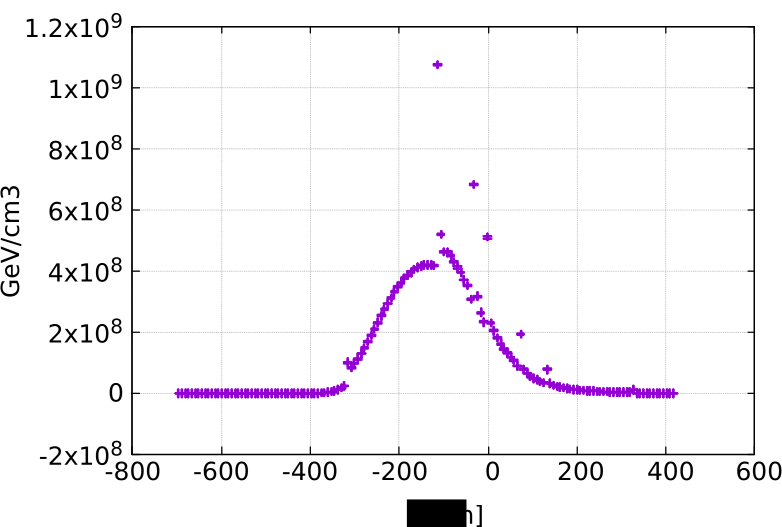
\includegraphics[height=0.248\textheight]{Figures/BeamDump/Energy_deposition_1DMax_z_Design2.png}
   \caption{\designtwo, z projection}
   \end{subfigure}
   \caption[Energy deposition in the ILC main beam dump]{\fluka result of the energy deposition density of one beam bunch in the ILC beam dump \designone (a) and \designtwo (b).
   The view is in the xz plane of the beam dump surrounding including the shielding walls.
   The color scale shows the deposited energy in \si{\GeV\per\centi\meter\cubed} per bunch.
   \\Figures (c) and (d) show the maximum values of the energy deposition as a projection on the z axis.}
   \label{fig:BeamDumps:Energy}
\end{figure}
\\Subfigures (c) and (d) show the projection of maximum values of the deposited energy onto the z axis.
The overall distribution of the deposited energy over z is smooth, with a maximum shortly before the vessel center.
Nevertheless, the distribution has several sharp peaks which can be identified to be at locations with large material density. \todo{English?!}
For \designone, the first sharp peak at z\,$\approx$\,\SI{-230}{\centi\meter} corresponds to the front side of the vortex tube, the back side of the same tube is also visible through the second peak at z\,$\approx$\,\SI{110}{\centi\meter}.
The third peak at z\,$\approx$\,\SI{220}{\centi\meter} is caused by the beam hitting the first copper plates in the end of the vessel.
\\Accordingly, the sharp peaks in Figure~\ref{fig:BeamDumps:Energy} (d) for \designtwo also correspond to locations with a higher material density.
The first two peaks at z\,$\approx$\,\SI{-100}{\centi\meter} and z\,$\approx$\,0 represent the high water pressure sections with their titanium tubes.
The last peak at z\,$\approx$\,\SI{120}{\centi\meter} originates from the first copper plates, which in this design are located closer to the vessel center.
\\The absolute value for the maximum energy deposited per bunch is between $\sim$\num{6.7e8} and \SI{1.1e9}{\GeV\per\centi\meter\cubed}, with the higher value for \designtwo.
 
\subsection{Dose}
\label{BeamDumps:sim_surrounding:Dose} 
From the deposited energy, \fluka can calculate the instantaneous dose equivalent of the beam dumps and their surrounding.
Figure~\ref{fig:BeamDumps:Dose} (a) and (b) show the \fluka results of the spatial distribution of the dose from one bunch in the xz plane, (c) and (d) show the projection of the maximum values onto the z axis, equivalent to the energy deposition plots before.
\\The distributions are comparable for both beam dump designs, the projection plots also again show sharp peaks at the locations of high material density.
The maximum dose equivalent from one bunch reaches about 82 - \SI{105}{\sievert}, with the higher value again for \designtwo.
\begin{figure}[h]
 \centering
  \begin{subfigure}[b]{0.49\textwidth}
   \centering
    \includegraphics[width=\textwidth]{Figures/BeamDump/Dose_equivalent_total_Design1.pdf}
   \caption{\designone, xz plane}
   \end{subfigure}
   \hfill
    \begin{subfigure}[b]{0.49\textwidth}
   \centering
    \includegraphics[width=\textwidth]{Figures/BeamDump/Dose_equivalent_total_Design2.pdf}
   \caption{\designtwo, xz plane}
   \end{subfigure}\\ \vspace*{0.3cm}
     \begin{subfigure}[b]{0.485\textwidth}
   \centering
    \includegraphics[height=0.24\textheight]{Figures/BeamDump/Dose_equivalent_total_1DMax_z_Design1.png}
   \caption{\designone, z projection}
   \end{subfigure}
   \hfill
    \begin{subfigure}[b]{0.485\textwidth}
   \centering
    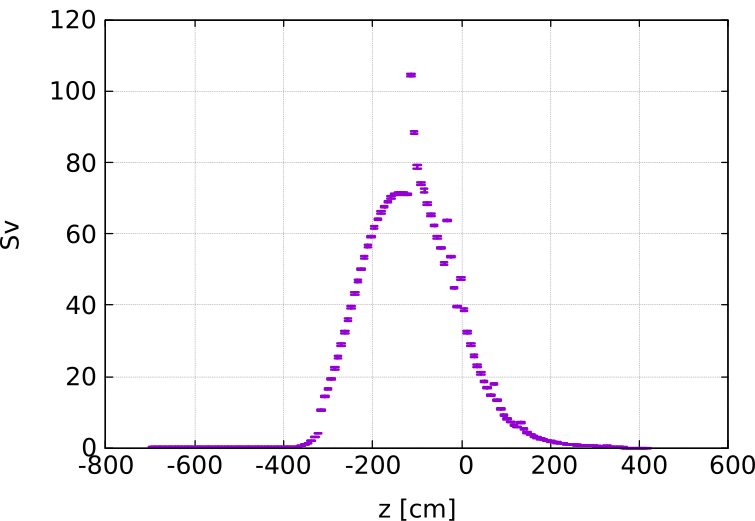
\includegraphics[height=0.24\textheight]{Figures/BeamDump/Dose_equivalent_total_1DMax_z_Design2.png}
   \caption{\designtwo, z projection}
   \end{subfigure}
   \caption[Dose equivalent in the ILC main beam dump]{\fluka result of the dose equivalent from one beam bunch in the ILC beam dump \designone (a) and \designtwo (b) and their surrounding.
   The view is in the xz plane of the beam dump surrounding including the shielding walls.
   The color scale shows the dose in \si{\milli\sievert} per bunch.
   \\Figures (c) and (d) show the maximum values of the dose as a projection on the z axis.
   The dose equivalent is here given in \si{\sievert}.}
   \label{fig:BeamDumps:Dose}
\end{figure}

From this, the remaining dose rate can be calculated after certain cooling times.
It was assumed that there has been full beam operation for one month, after which the accelerator is turned off.
Considering the cooling times of one minute, one hour, one day, one month, and one year after the moment of the beam operation stop, the remaining dose rate decreases over time.
Figure~\ref{fig:BeamDumps:DoseRate} shows the spatial distribution of the dose rate for \designone and \designtwo for the cooling times mentioned above.
The comparison of the dose rate as a function of the cooling time for the two designs is then given in Figure~\ref{fig:BeamDumps:DoseRate_Comparison}.
\\Even after one minute of cooling time the area in which a dose is measurable is reduced to the beam dump vessel and the direct surrounding.
Over the duration of one year the dose is decreasing by at least two orders of magnitude.
Nevertheless, the maximum dose rate after one year is about \SI{0.1}{\milli\sievert\per\second} for \designone, and \SI{10}{\milli\sievert\per\second} for \designtwo.
For a given legal dose limit of \SI{50}{\milli\sievert} per year for workers whose work involves radiation activities, maintenance personnel would be allowed to work on the beam dump vessel for a very restricted time only.
\\The residual nuclei, which are the cause for the high dose rates, are shown in Figure~\ref{fig:BeamDumps:ResidualNuclei}.
The main contributors are \textsuperscript{3}H (tritium), \textsuperscript{49}V, \textsuperscript{54}Mn, \textsuperscript{55}Fe, \textsuperscript{56}Co, \textsuperscript{57}Co, \textsuperscript{58}Co, and \textsuperscript{60}Co, with a half-life between $\sim$1 and 13 years.

\begin{figure}[hbp]
\centering
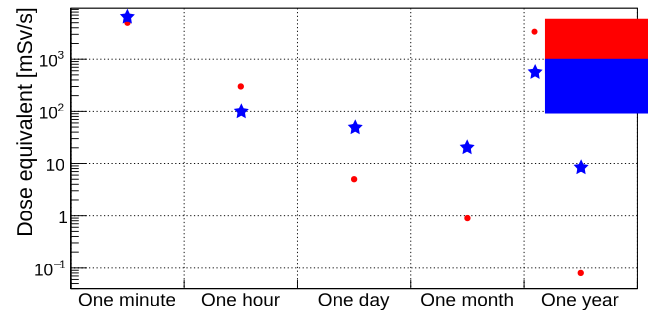
\includegraphics[width=0.65\textwidth]{Figures/BeamDump/DoseEQ_Time_Comparison.png}
\caption[Dose rate comparison of the ILC main beam dump designs]{Comparison of the maximum dose rate over the cooling time for the two ILC main beam dump designs \designone and \designtwo.}
\label{fig:BeamDumps:DoseRate_Comparison}
\end{figure}

\begin{figure}[hbp]
\centering
\includegraphics[width=0.6\textwidth]{Figures/BeamDump/Corrected_residualnuclei_plots/ResidualNuclei_Design2_5_correct_scale.pdf}
\caption[Residual nuclei in the ILC main beam dump after one year]{Chart of residual nuclei in the beam dump vessel and its surrounding after a cooling time of one year.
The axes show the number of protons (Z) and the number of neutrons (N) of the nuclei, from which the according element can be derived.
The color scale indicates the radioactivity in \si{\becquerel\per\centi\meter\cubed} of the respective nuclei.}
\label{fig:BeamDumps:ResidualNuclei}
\end{figure}

\begin{figure}[!h]
 \centering
  \begin{subfigure}[b]{0.32\textwidth}
   \centering
    \includegraphics[width=\textwidth]{Figures/BeamDump/Design1_1.png}
   \caption{\designone, 1 minute}
   \end{subfigure}
   \hfill
    \begin{subfigure}[b]{0.32\textwidth}
   \centering
    \includegraphics[width=\textwidth]{Figures/BeamDump/Design1_2.png}
   \caption{\designone, 1 hour}
   \end{subfigure}
      \hfill
     \begin{subfigure}[b]{0.32\textwidth}
   \centering
    \includegraphics[width=\textwidth]{Figures/BeamDump/Design1_3.png}
   \caption{\designone, 1 day}
   \end{subfigure}\\ 
    \begin{subfigure}[b]{0.32\textwidth}
   \centering
    \includegraphics[width=\textwidth]{Figures/BeamDump/Design1_4.png}
   \caption{\designone, 1 month}
   \end{subfigure}
      \hfill
    \begin{subfigure}[b]{0.32\textwidth}
   \centering
    \includegraphics[width=\textwidth]{Figures/BeamDump/Design1_5.png}
   \caption{\designone, 1 year}
   \end{subfigure} 
   \hfill
   \begin{minipage}{0.32\textwidth}
   \hfill
    \end{minipage}
   \\
     \begin{subfigure}[b]{0.32\textwidth}
   \centering
    \includegraphics[width=\textwidth]{Figures/BeamDump/Design2_1.png}
   \caption{\designtwo, 1 minute}
   \end{subfigure}
   \hfill
    \begin{subfigure}[b]{0.32\textwidth}
   \centering
    \includegraphics[width=\textwidth]{Figures/BeamDump/Design2_2.png}
   \caption{\designtwo, 1 hour}
   \end{subfigure}
      \hfill
     \begin{subfigure}[b]{0.32\textwidth}
   \centering
    \includegraphics[width=\textwidth]{Figures/BeamDump/Design2_3.png}
   \caption{\designtwo, 1 day}
   \end{subfigure}\\
    \begin{subfigure}[b]{0.32\textwidth}
   \centering
    \includegraphics[width=\textwidth]{Figures/BeamDump/Design2_4.png}
   \caption{\designtwo, 1 month}
   \end{subfigure}
      \hfill
    \begin{subfigure}[b]{0.32\textwidth}
   \centering
    \includegraphics[width=\textwidth]{Figures/BeamDump/Design2_5.png}
   \caption{\designtwo, 1 year}
   \end{subfigure}
   \hfill
   \begin{minipage}{0.32\textwidth}
   \hfill
    \end{minipage}
   \caption[Dose rate in the ILC main beam dump after cooling times]{\fluka result of the dose rate in the ILC beam dump \designone (a) and \designtwo (b) and their surrounding after one month of beam operation and certain cooling times.
   The cooling times are given in the captions of the individual subfigures.
   The view is in the xz plane of the beam dump surrounding including the shielding walls.
   The color scale shows the dose rate in \si{\milli\sievert\per\second}.}
   \label{fig:BeamDumps:DoseRate}
\end{figure}
 
\subsection{Particle fluxes}
\label{BeamDumps:sim_surrounding:Particle}  
 The densities of particles in the geometry can also be scored with \fluka, which is then given as the number of particles per \si{\centi\meter\cubed}.
 As an example, Figure~\ref{fig:BeamDumps:Electrons} shows the density distribution of electrons in the xz plane for the two ILC beam dump designs.
 Since the primary beam also consists of electrons, the beam path is also visible coming from negative z along the beam pipe.
 Inside the water vessel, the beam is stopped and dissipated, and particle showers start forming. The electrons are boosted in the beam direction, because of which electrons outside the beam dump are mainly observed around and behind the vessel. 
 \\This looks quite different for the neutron density distributions (Figure~\ref{fig:BeamDumps:Neutrons}).
 The primary electron beam undergoes the electromagnetic particle showers in the beam dump, which is desired in order to absorb the beam power.
 The produced secondary particles from the particle showers, however, interact with the beam dump material and the water via ionization and photonuclear processes.
 The products from these processes are neutrons in connection with the radioactive nuclei discussed in Section~\ref{BeamDumps:sim_surrounding:Dose}.
 Due to this way of production, the neutrons can be found under every solid angle, hence also in the backward direction. \todo{English?!}
 
\begin{figure}[h]
 \centering
  \begin{subfigure}[b]{0.49\textwidth}
   \centering
    \includegraphics[width=\textwidth]{Figures/BeamDump/Electron_flux_xz_Design1.png}
   \caption{\designone}
   \end{subfigure}
   \hfill
    \begin{subfigure}[b]{0.49\textwidth}
   \centering
    \includegraphics[width=\textwidth]{Figures/BeamDump/Electron_flux_xz_Design2.png}
   \caption{\designtwo}
   \end{subfigure}
   \caption[Electron flux in the ILC main beam dump]{\fluka result of the electron flux from one beam bunch in the ILC beam dump \designone (a) and \designtwo (b) and their surrounding.
   The view is in the xz plane of the beam dump.
   The color scale shows the dose in number of particles per \si{\centi\meter\cubed} per bunch.}
   \label{fig:BeamDumps:Electrons}
\end{figure} 

\begin{figure}[h]
 \centering
  \begin{subfigure}[b]{0.49\textwidth}
   \centering
    \includegraphics[width=\textwidth]{Figures/BeamDump/Neutron_flux_xz_Design1.png}
   \caption{\designone}
   \end{subfigure}
   \hfill
    \begin{subfigure}[b]{0.49\textwidth}
   \centering
    \includegraphics[width=\textwidth]{Figures/BeamDump/Neutron_flux_xz_Design2.png}
   \caption{\designtwo}
   \end{subfigure}
   \caption[Neutron flux in the ILC main beam dump]{\fluka result of the neutron flux from one beam bunch in the ILC beam dump \designone (a) and \designtwo (b) and their surrounding.
   The view is in the xz plane of the beam dump.
   The color scale shows the dose in number of particles per \si{\centi\meter\cubed} per bunch.}
   \label{fig:BeamDumps:Neutrons}
\end{figure} 

Neutron spatial distributions

\section{Simulation studies of extraction line}
\label{BeamDumps:sim_EXT}

\begin{itemize}
 \item Extraction line lattice - explain components
 \item Simulation of neutrons through EXT - not done yet
\end{itemize}

\section{SiD Occupancy study from beam dump neutrons}
\label{BeamDumps:SiDocc}

\begin{itemize}
 \item Occupancy study of neutrons in SiD - not done yet
\end{itemize}